%%%%%%%%%%%%%%%%%%%%%%%%%%%%%%%%%%%%%%%%%
% Beamer Presentation
% LaTeX Template
% Version 1.0 (10/11/12)
%
% This template has been downloaded from:
% http://www.LaTeXTemplates.com
%
% License:
% CC BY-NC-SA 3.0 (http://creativecommons.org/licenses/by-nc-sa/3.0/)
%
%%%%%%%%%%%%%%%%%%%%%%%%%%%%%%%%%%%%%%%%%

%----------------------------------------------------------------------------------------
%	PACKAGES AND THEMES
%----------------------------------------------------------------------------------------

\documentclass{beamer}

\mode<presentation> {

% The Beamer class comes with a number of default slide themes
% which change the colors and layouts of slides. Below this is a list
% of all the themes, uncomment each in turn to see what they look like.

%\usetheme{default}
%\usetheme{AnnArbor}
%\usetheme{Antibes}
%\usetheme{Bergen}
%\usetheme{Berkeley}
%\usetheme{Berlin}
%\usetheme{Boadilla}
%\usetheme{CambridgeUS}
%\usetheme{Copenhagen}
%\usetheme{Darmstadt}
%\usetheme{Dresden}
%\usetheme{Frankfurt}
%\usetheme{Goettingen}
%\usetheme{Hannover}
%\usetheme{Ilmenau}
%\usetheme{JuanLesPins}
%\usetheme{Luebeck}
%\usetheme{Madrid}
%\usetheme{Malmoe}
%\usetheme{Marburg}
%\usetheme{Montpellier}
%\usetheme{PaloAlto}
%\usetheme{Pittsburgh}
%\usetheme{Rochester}
%\usetheme{Singapore}
%\usetheme{Szeged}
\usetheme{Warsaw}

%\usecolortheme{albatross}
%\usecolortheme{beaver}
%\usecolortheme{beetle}
%\usecolortheme{crane}
%\usecolortheme{dolphin}
%\usecolortheme{dove}
%\usecolortheme{fly}
%\usecolortheme{lily}
%\usecolortheme{orchid}
%\usecolortheme{rose}
%\usecolortheme{seagull}
\usecolortheme{seahorse}
%\usecolortheme{whale}
%\usecolortheme{wolverine}

\usefonttheme{professionalfonts} 
\setbeamertemplate{caption}[numbered]
%\usetheme{}

\addtobeamertemplate{navigation symbols}{}{%
    \usebeamerfont{footline}%
    \usebeamercolor[fg]{footline}%
    \hspace{1em}%
    \insertframenumber/\inserttotalframenumber
}

\usepackage[utf8]{inputenc}
\usepackage[english]{babel}
\usepackage{physics}
\usepackage{amsmath}
\usepackage{bm}
\usepackage{amsfonts}
\usepackage{amssymb}
\usepackage{caption}
\usepackage{subcaption}
\usepackage{float}

%\setbeamertemplate{footline} % To remove the footer line in all slides uncomment this line
%\setbeamertemplate{footline}[page number] % To replace the footer line in all slides with a simple slide count uncomment this line

%\setbeamertemplate{navigation symbols}{} % To remove the navigation symbols from the bottom of all slides uncomment this line
}

\usepackage{graphicx} % Allows including images
\usepackage{booktabs} % Allows the use of \toprule, \midrule and \bottomrule in tables

%----------------------------------------------------------------------------------------
%	TITLE PAGE
%----------------------------------------------------------------------------------------

\title[2. Airbounce]{Problem no.2 - Airbounce}
\subtitle{IPT 2022}
\author[University of Ljubljana]{Team Slovenia \\ Presenter: Rok Grgi\v c Me\v sko}
\date{\vspace{-5ex}}

\begin{document}

\begin{frame}

\begin{figure}[H]
	\centering
	  
\includegraphics[width=\textwidth]{naslovnica_ipt.png}
\end{figure}

\titlepage % Print the title page as the first slide

\vspace{-13mm}
\begin{figure}[H]
	\flushleft
	  
\includegraphics[width=6cm]{fmf_logo.png}
\end{figure}

\end{frame}


%----------------------------------------------------------------------------------------
%	PRESENTATION SLIDES
%----------------------------------------------------------------------------------------

%------------------------------------------------


\begin{frame}

\begin{block}{Official Problem Statement}
When a Frisbee is thrown in a certain way it can be made to bounce in mid-air. Study the physics of this phenomenon.
\end{block}
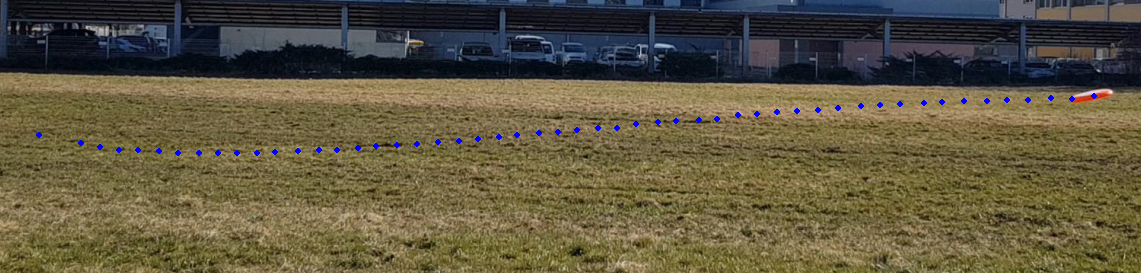
\includegraphics[width=\textwidth]{primer_meta.png}

\end{frame}

%------------------------------------------------

\begin{frame}

\begin{block}{Ideas and Hypotheses}
\begin{itemize}
\item Normal component of Frisbee velocity will decrease faster because of its shape.

\item Frisbee will appear to bounce in mid-air.
\end{itemize}
\end{block}

\end{frame}

%------------------------------------------------

\begin{frame}

\frametitle{Theoretical Description}

\begin{block}{}
\begin{itemize}
\item Frisbee in the original video is stable. Angle to the ground is constant.

\item Assumptions:

\begin{itemize}
\item Frisbee keeps constant angle to the ground during the whole flight because of gyroscopic stability.

\item Frisbee travels in a straight line. (no Magnus effect...)
\end{itemize}
\end{itemize}
\end{block}

\end{frame}

%------------------------------------------------

\begin{frame}

\frametitle{Theoretical Description}

\begin{Large}
Axis graphs:
\end{Large}

\begin{figure}[H]
	\centering
	\begin{minipage}{.5\textwidth}
	  \centering
	  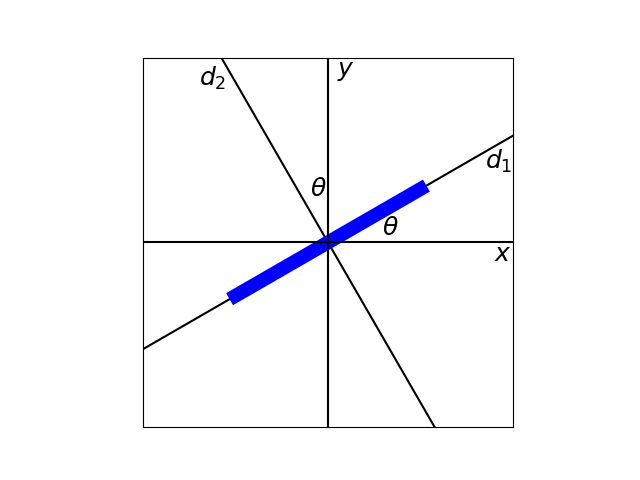
\includegraphics[width=\textwidth]{graf_osi.png}
	  \captionof{figure}{\\ Ground coordinate system: N}
	\end{minipage}%
	\begin{minipage}{.5\textwidth}
	  \centering
	  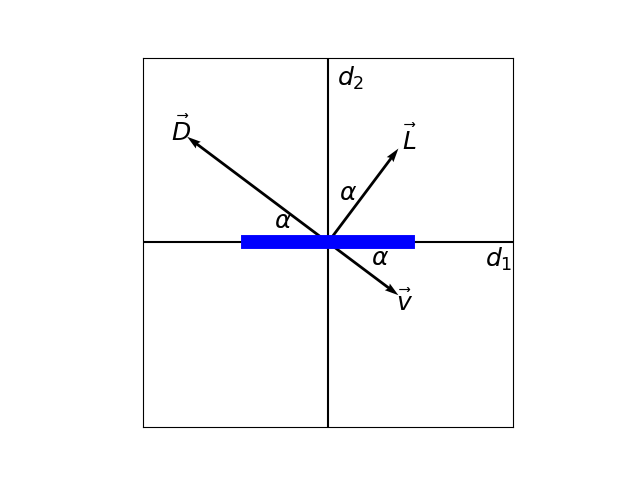
\includegraphics[width=\textwidth]{osi_frisbeeja.png}
	  \captionof{figure}{\\ Coordinate system of Frisbee: D}
	\end{minipage}
\end{figure}

$ \theta = $ angle to the ground \qquad \qquad $ \alpha = $ angle of attack

\end{frame}

%------------------------------------------------

\begin{frame}

\frametitle{Theoretical Description}

\begin{block}{Lift and drag force}
\begin{equation}
L = \dfrac{1}{2} A \rho C_L v^2 \qquad D = \dfrac{1}{2} A \rho C_D v^2
\end{equation}
\end{block}

\begin{block}{Lift and drag coefficient depending on angle of attack \cite{clanek}}
\begin{equation}
C_L = C_{L0} + C_{L \alpha} \alpha \qquad C_D = C_{D0} + C_{D \alpha} \alpha^2
\end{equation}
\end{block}

\end{frame}

%------------------------------------------------

\begin{frame}

\frametitle{Theoretical Description}

\begin{block}{Cutoff}
\begin{itemize}
\item $C_D$ cutoff; when $C_D = 1.1$ (drag coefficient of a disc perpendicular to velocity)

\item $C_L$ cutoff; at stall angle = $25^{\circ}$
\end{itemize}
\end{block}

\begin{figure}[H]
	\centering	  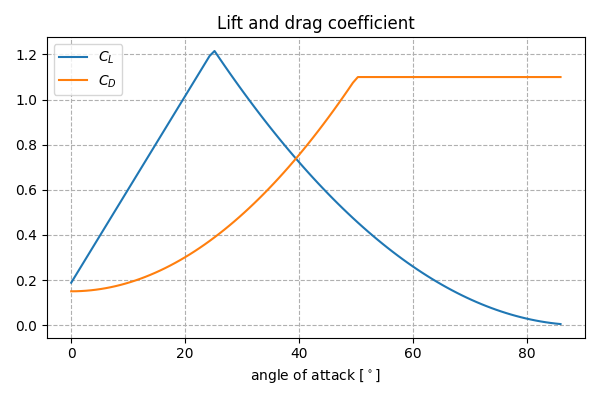
\includegraphics[width=0.5\textwidth]{lift_drag_primer.png}
	  \caption{$C_{L0} = 0.188, C_{L \alpha}= 2.37, C_{D0} = 0.15, C_{D \alpha} = 1.24$  \\	M. Hubbard, S. A. Hummel. \textit{Simulation of Frisbee Flight}. (2000). \cite{clanek}  (short flights)}
\end{figure}

\end{frame}

%------------------------------------------------

\begin{frame}

\frametitle{Theoretical Description: Forces}

\begin{columns}[onlytextwidth]

\column{0.5 \textwidth}

\vspace{-10mm}
\begin{figure}[H]
	\centering
	  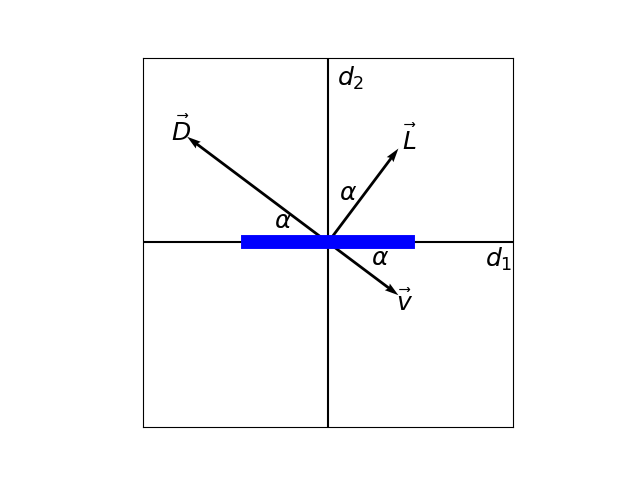
\includegraphics[width=\textwidth]{osi_frisbeeja.png}
	  \caption{Coordinate system of Frisbee: D}
\end{figure}

\vspace{-10mm}
\begin{gather*}
K = \dfrac{A \rho}{2 m} \qquad \tan \alpha = \dfrac{-v_2}{v_1}\\
v = \sqrt{v_1^2 + v_2^2}
\end{gather*}

\column{0.5 \textwidth}

\vspace{-10mm}

\begin{gather}
\begin{split}
\bm L = m K C_L v^2 \mqty(\sin \alpha \\ \cos \alpha)_D\\
\bm L = m K  C_L v \mqty(-v_2 \\ v_1\\)_D
\end{split}
\end{gather}

\begin{gather}
\begin{split}
\bm D = m K C_D v^2 \mqty(-\cos \alpha \\ \sin \alpha)_D\\
\bm D = m K C_D v \mqty(-v_1 \\ -v_2\\)_D
\end{split}
\end{gather}

\begin{gather}
\begin{split}
\bm F_{\bm g} = - m g  \mqty(\sin \theta \\ \cos \theta)_D
\end{split}
\end{gather}

\end{columns}

\end{frame}

%------------------------------------------------

\begin{frame}

\frametitle{Theoretical Description}

\begin{gather}
m \bm a = \bm L + \bm D + \bm F_{\bm g}\\
\mqty( \dot{v_1} \\ \dot{v_2}\\)_D = K  C_L v \mqty(-v_2 \\ v_1\\)_D + K C_D v \mqty(-v_1 \\ -v_2\\)_D - g  \mqty(\sin \theta \\ \cos \theta)_D\\
%a_1 = -K (C_{L0} + C_{L \alpha} \alpha) v v_2 - K (C_{D0} + C_{D \alpha} \alpha^2) v v_1 - g \sin \theta\\
%a_2 = K (C_{L0} + C_{L \alpha} \alpha) v v_1 - K (C_{D0} + C_{D \alpha} \alpha^2) v v_2 - g \cos\theta
\mqty( \dot{d_1} \\ \dot{d_2}\\)_D = \mqty( v_1 \\v_2\\)_D
\end{gather}
Solve for: $d_1, d_2, v_1, v_2 $ and rotate to ground coordinate system N.
\begin{gather}
R = \mqty(\cos \theta & -\sin \theta \\ \sin \theta & \cos \theta)\\
\mqty(x \\ y)_N = R \mqty(d_1 \\ d_2)_D \qquad \mqty(v_x \\ v_y)_N = R \mqty(v_1 \\ v_2)_D
\end{gather}
\end{frame}

%------------------------------------------------

\begin{frame}

\frametitle{Experiment}

\begin{itemize}
\item Video analysis of a throw.
\item Analysed only stable throws.
\item Problems:

\begin{itemize}
\item Frisbee is not stable as in the original video.
\item Parallax error. Throw is not perpendicular to the camera.
\item Wind speed was not measured.
\item Rotation of Frisbee not measured, coefficients of lift and drag for rotating Frisbee.
\end{itemize}

\end{itemize}

\end{frame}

%------------------------------------------------

\begin{frame}

\frametitle{Experiment}

\begin{table}
\begin{tabular}{|c|c|c|c|c|c|}
\hline 
$m [\mathrm{kg}]$ & $A [\mathrm{m^2}]$ & $\rho [\mathrm{kg/m^3}]$ &  $g [\mathrm{m / s^2}]$ \\ 
\hline 
$0.175$ & $0.0616$ & $1.23$ & $9.8$ \\ 
\hline 
\end{tabular}
\caption{Frisbee parameters and constants.}
\end{table} 

\begin{figure}[H]
	\centering
	  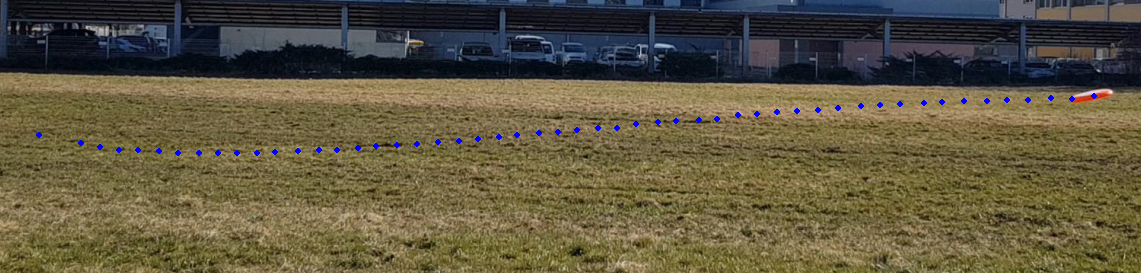
\includegraphics[width=\textwidth]{primer_meta.png}
	  \caption{Example of a throw.}
\end{figure}

\end{frame}

%------------------------------------------------

\begin{frame}

\frametitle{Parallax Error Correction}

\(dx\) is measured, \(dx'\) is correct

\begin{gather}
k = \dfrac{\mathrm{final \; frisbee \; size}}{\mathrm{initial \;  frisbee  \; size}} \qquad l = \mathrm{lenght \; of \; a \; throw}\\
dx = \left( \dfrac{k - 1}{l} x + 1 \right) dx' \\
x' = \int_{0}^{x} \left( \dfrac{k - 1}{l} x + 1 \right)^{-1} \,dx \\
x' = \dfrac{l}{k - 1} \left[ \ln((k - 1) x + l) - \ln l \right]
\end{gather}

\end{frame}

%------------------------------------------------

\begin{frame}

\frametitle{Results, example of a throw:}

\begin{figure}[H]
	\centering
	  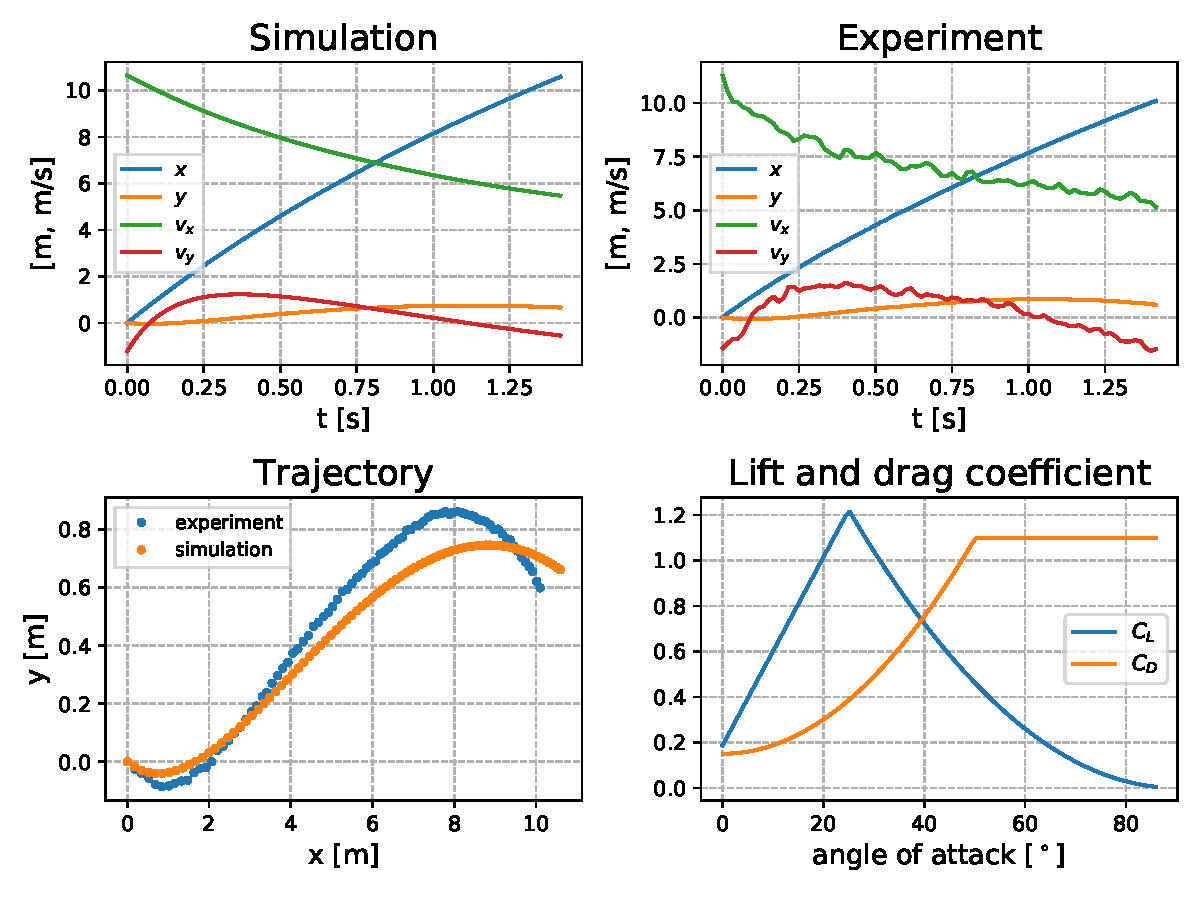
\includegraphics[width=0.85 \textwidth]{strmo_clanek_vse.pdf}
	  \captionsetup{justification=centering,margin=0cm}
	  \caption{$\theta = 19 ^{\circ}$, $v_x(t = 0) = 10.64 \mathrm{\frac{m}{s}}$, $v_y(t = 0) = -1.21 \mathrm{\frac{m}{s}}$ \\
	  $C_L, C_D$: article \cite{clanek}}
\end{figure}


\end{frame}

%------------------------------------------------

\begin{frame}

\frametitle{Fitting $C_L$ and $C_D$}

Angle to the ground ($\theta$) in not constant, we used effective (average) angle $\theta_{ef}$.\\
Parameters in finding $C_L$ and $C_D$:\\
 \quad	$\theta_{ef}$, $C_{L0}$, $C_{L \alpha}$, $C_{D0}$, $C_{D \alpha}$

\begin{block}{Minimization of $s$ over $k$ experiments:}
\begin{gather}
s_k = \sum_{i} w_i \, \| (x_i, y_i)_{sim} - (x_i, y_i)_{exp} \|^2 \\
s = \sum_k s_k\\
w_i = \dfrac{1}{\Delta x_i^2}
\end{gather}

\begin{center}
\texttt{scipy.optimize.minimize(method='TNC')}
\end{center}
\end{block}

\end{frame}

%------------------------------------------------

\begin{frame}

\frametitle{Fitting $C_L$ and $C_D$}

\begin{block}{Weights}
\begin{gather}
x_i = \int_{0}^{t_i} \left( \int_{0}^{t_i} a \, dt \right) \,dt \\
\Delta x_i = \pdv{x_i}{a} \Delta a + \Delta x_0\\
w_i = \left( \dfrac{\Delta a}{2} \, t_i^2 + \Delta x_0 \right)^{-2}
\end{gather}
\end{block}

\[ \Delta a \approx 0.1 \mathrm{\dfrac{m}{s^2}} \qquad \Delta x_0 \approx 1 \mathrm{cm} \]

\end{frame}
%------------------------------------------------

\begin{frame}

\frametitle{Fitting $C_L$ and $C_D$}

\begin{figure}[H]
	\centering
	  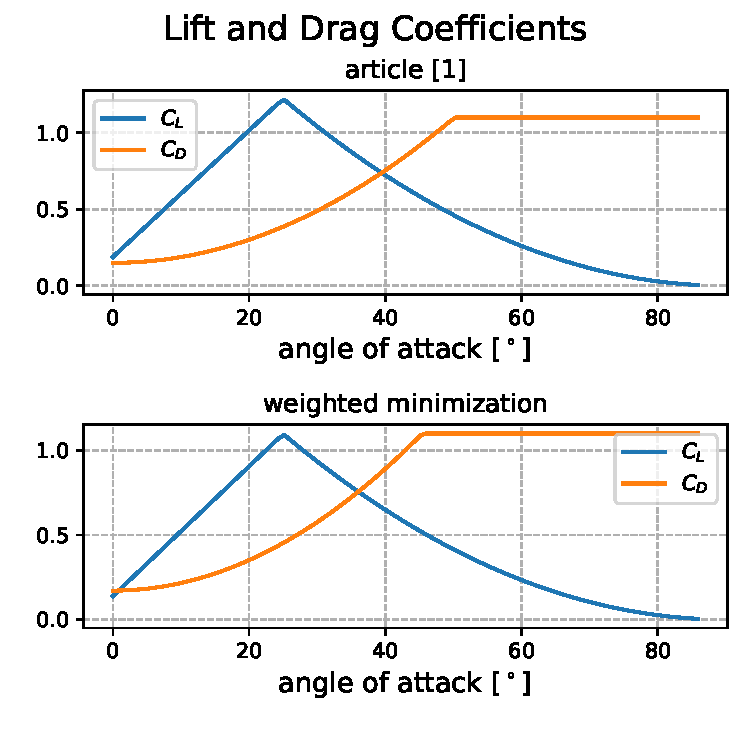
\includegraphics[width=0.6 \textwidth]{cji_clanek_weighted.pdf}
	  \captionsetup{justification=centering,margin=0cm}
	  \caption{$C_{L0} = 0.188, C_{L \alpha}= 2.37, C_{D0} = 0.15, C_{D \alpha} = 1.24$ \cite{clanek} \\
	  $C_{L0} = 0.138, C_{L \alpha}= 2.20, C_{D0} = 0.171, C_{D \alpha} = 1.47$ [minimization]}
\end{figure}

\end{frame}

%------------------------------------------------
\begin{frame}

\begin{figure}[H]
	\centering
	  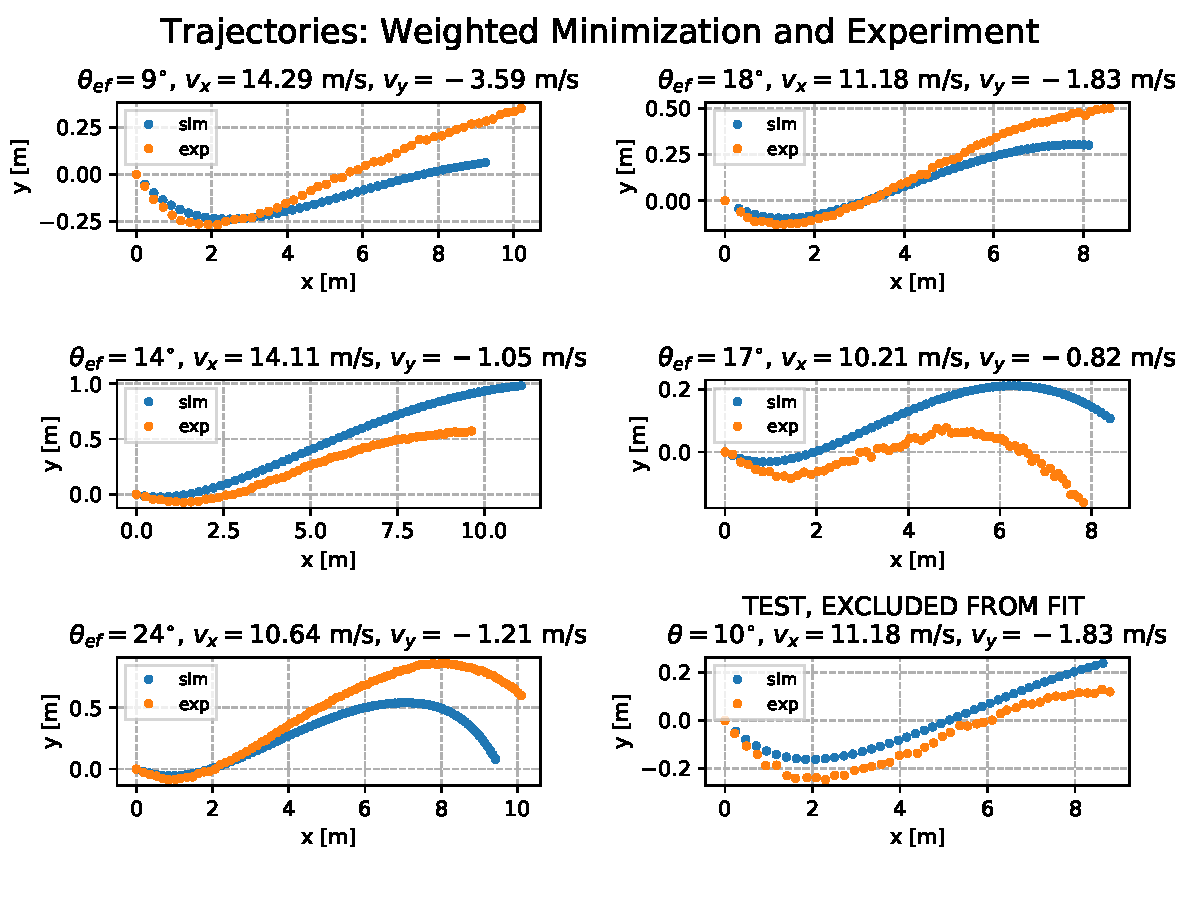
\includegraphics[width= \textwidth]{traj_weighted_mini.pdf}
	  \captionsetup{justification=centering,margin=0cm}
	  \caption{All experiments.}
\end{figure}

\end{frame}

%------------------------------------------------

\begin{frame}

\frametitle{Minimization: Weighted vs Unweighted }

\begin{figure}[H]
	\centering
	  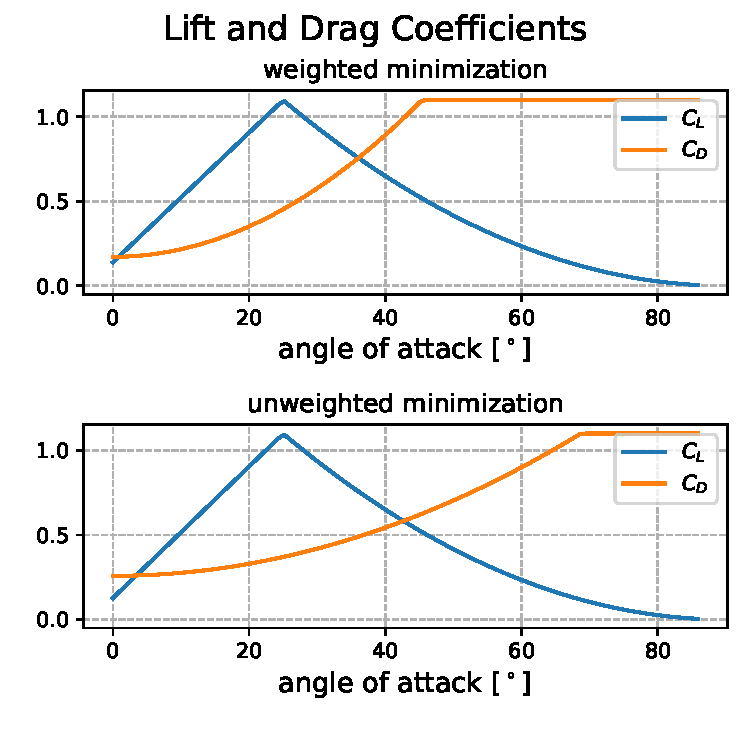
\includegraphics[width=0.6 \textwidth]{cji_weighted_unweighted.pdf}
	  \captionsetup{justification=centering,margin=0cm}
	  \caption{$C_{L0} = 0.138, C_{L \alpha}= 2.20, C_{D0} = 0.171, C_{D \alpha} = 1.47 \,$(weighted) \\
	  $C_{L0} = 0.127, C_{L \alpha}= 2.23, C_{D0} = 0.258, C_{D \alpha} = 0.585 \,$(unweighted) }
\end{figure}

\end{frame}

%------------------------------------------------
\begin{frame}

\begin{figure}[H]
	\centering
	  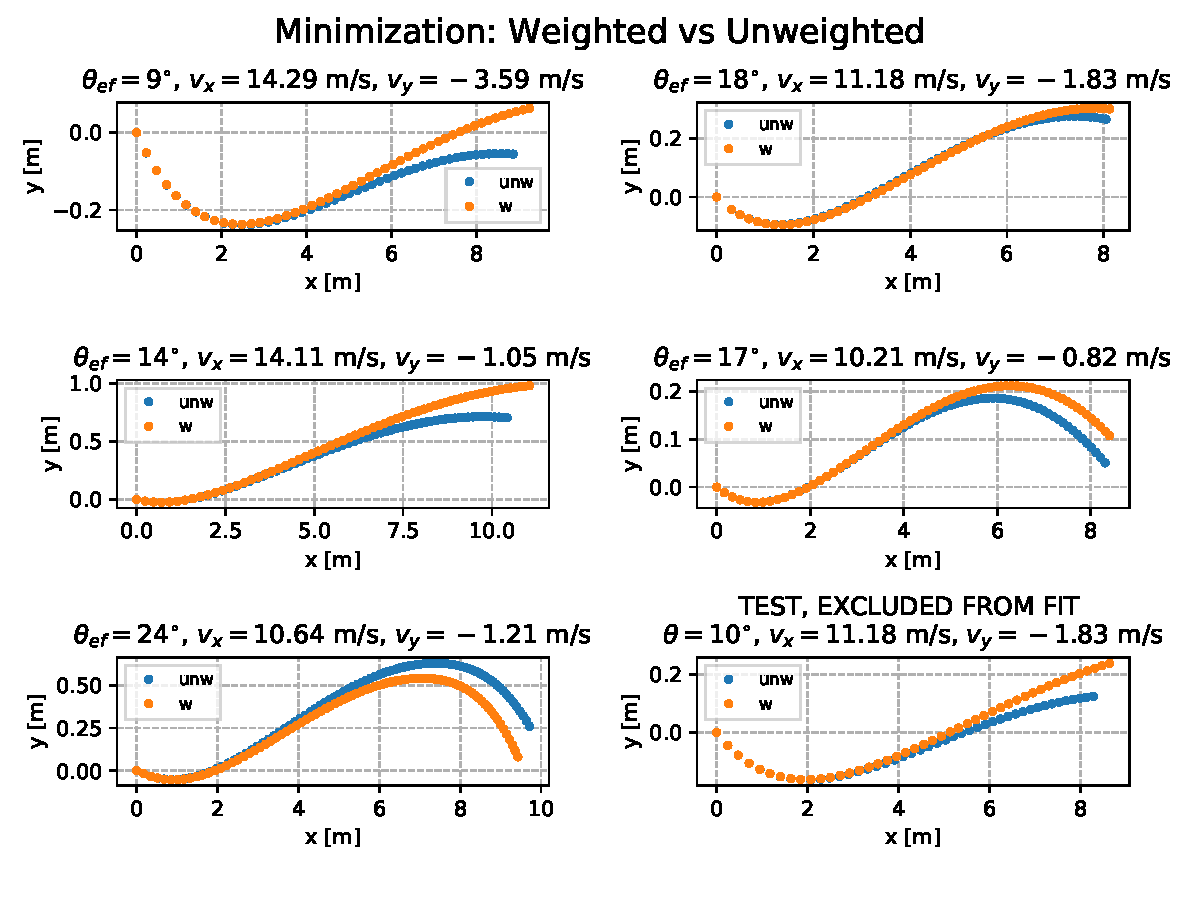
\includegraphics[width= \textwidth]{traj_unweighted_weighted.pdf}
	  \captionsetup{justification=centering,margin=0cm}
	  \caption{All experiments.}
\end{figure}

\end{frame}

%------------------------------------------------

\begin{frame}

\frametitle{Nondimensionalization}

\begin{gather}
t = T_c \tau,  \quad d_i = D_c \sigma_i, \quad v_i = \dfrac{D_c}{T_c} \, \nu_i, \quad
\dot{v_i} = \dfrac{D_c}{T_c^2} \, \nu_i'
\\
\mqty( \dot{v_1} \\ \dot{v_2}\\)_D = K  C_L v \mqty(-v_2 \\ v_1\\)_D + K C_D v \mqty(-v_1 \\ -v_2\\)_D - g  \mqty(\sin \theta \\ \cos \theta)_D
\end{gather}
$$\Downarrow$$
\begin{gather}
\mqty( \nu_1' \\ \nu_2' \\)_D = C_L  \, \nu \mqty(-\nu_2 \\ \nu_1\\)_D + C_D \, \nu \mqty(-\nu_1 \\ -\nu_2\\)_D -   \mqty(\sin \theta \\ \cos \theta)_D
\\
D_c = \dfrac{2m}{A \rho} = 4.6 \mathrm{m}, \quad T_c = \sqrt{\dfrac{2m}{A \rho g}} = 0.68 \mathrm{s}
\end{gather}

\end{frame}

%------------------------------------------------

\begin{frame}

\frametitle{Bounce part without gravity}
Only $\alpha$ (angle of attack) and $v$ remain as initial parameters.

\begin{gather}
D_c = \dfrac{2m}{A \rho}, \quad T_c = 1 \mathrm{s}
\\
\mqty( \nu_1' \\ \nu_2' \\) = C_L  \, \nu \mqty(-\nu_2 \\ \nu_1\\) + C_D \, \nu \mqty(-\nu_1 \\ -\nu_2\\)
\end{gather}
Changing initial speed only scales in time, trajectory shape is the same.

\vspace{-3mm}

\begin{figure}[H]
	\centering
	  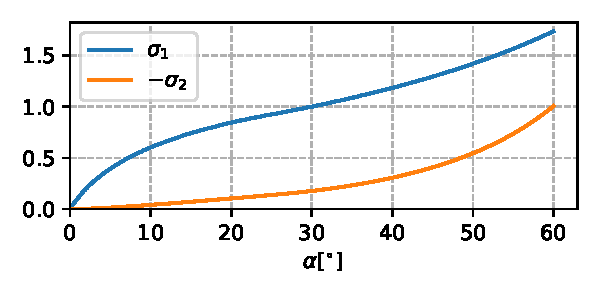
\includegraphics[width= 0.6\textwidth]{distance_to_bounce.pdf}
	  \captionsetup{justification=centering,margin=0cm}
	  \caption{Distance and depth to the bounce minimum with angle of attack.}
\end{figure}


\end{frame}

%------------------------------------------------

\begin{frame}

\frametitle{Phase diagram}


\end{frame}

%------------------------------------------------

\begin{frame}

\frametitle{Conclusion}

\begin{itemize}
\item Simulation and experiment match.
\item Coefficients similar as article: good model
\item Experiment improvements:

\begin{itemize}
\item measure wind speed 
\item practice more for a stable throw
\item experiment conducted inside
\item measure Frisbee rotation
\end{itemize}

\end{itemize}

\end{frame}

%------------------------------------------------

\begin{frame}

\frametitle{References}

\setbeamertemplate{bibliography item}[text]

\begin{thebibliography}{9}

\bibitem{clanek}
M. Hubbard, S. A. Hummel. \textit{Simulation of Frisbee Flight}. (2000). \url{https://www.researchgate.net/publication/253842372_Simulation_of_Frisbee_Flight}

\bibitem{clanekPC}
J. Potts, W. J. Crowther. \textit{Disc-wing Aerodynamics}. (2002). \url{https://www.researchgate.net/publication/268559957_FrisbeeTM_Aerodynamics}

\end{thebibliography}

\end{frame}

%------------------------------------------------

\end{document} 